% Options for packages loaded elsewhere
\PassOptionsToPackage{unicode}{hyperref}
\PassOptionsToPackage{hyphens}{url}
%
\documentclass[
]{article}
\usepackage{amsmath,amssymb}
\usepackage{lmodern}
\usepackage{iftex}
\ifPDFTeX
  \usepackage[T1]{fontenc}
  \usepackage[utf8]{inputenc}
  \usepackage{textcomp} % provide euro and other symbols
\else % if luatex or xetex
  \usepackage{unicode-math}
  \defaultfontfeatures{Scale=MatchLowercase}
  \defaultfontfeatures[\rmfamily]{Ligatures=TeX,Scale=1}
\fi
% Use upquote if available, for straight quotes in verbatim environments
\IfFileExists{upquote.sty}{\usepackage{upquote}}{}
\IfFileExists{microtype.sty}{% use microtype if available
  \usepackage[]{microtype}
  \UseMicrotypeSet[protrusion]{basicmath} % disable protrusion for tt fonts
}{}
\makeatletter
\@ifundefined{KOMAClassName}{% if non-KOMA class
  \IfFileExists{parskip.sty}{%
    \usepackage{parskip}
  }{% else
    \setlength{\parindent}{0pt}
    \setlength{\parskip}{6pt plus 2pt minus 1pt}}
}{% if KOMA class
  \KOMAoptions{parskip=half}}
\makeatother
\usepackage{xcolor}
\usepackage[margin=1in]{geometry}
\usepackage{longtable,booktabs,array}
\usepackage{calc} % for calculating minipage widths
% Correct order of tables after \paragraph or \subparagraph
\usepackage{etoolbox}
\makeatletter
\patchcmd\longtable{\par}{\if@noskipsec\mbox{}\fi\par}{}{}
\makeatother
% Allow footnotes in longtable head/foot
\IfFileExists{footnotehyper.sty}{\usepackage{footnotehyper}}{\usepackage{footnote}}
\makesavenoteenv{longtable}
\usepackage{graphicx}
\makeatletter
\def\maxwidth{\ifdim\Gin@nat@width>\linewidth\linewidth\else\Gin@nat@width\fi}
\def\maxheight{\ifdim\Gin@nat@height>\textheight\textheight\else\Gin@nat@height\fi}
\makeatother
% Scale images if necessary, so that they will not overflow the page
% margins by default, and it is still possible to overwrite the defaults
% using explicit options in \includegraphics[width, height, ...]{}
\setkeys{Gin}{width=\maxwidth,height=\maxheight,keepaspectratio}
% Set default figure placement to htbp
\makeatletter
\def\fps@figure{htbp}
\makeatother
\setlength{\emergencystretch}{3em} % prevent overfull lines
\providecommand{\tightlist}{%
  \setlength{\itemsep}{0pt}\setlength{\parskip}{0pt}}
\setcounter{secnumdepth}{-\maxdimen} % remove section numbering
\ifLuaTeX
  \usepackage{selnolig}  % disable illegal ligatures
\fi
\IfFileExists{bookmark.sty}{\usepackage{bookmark}}{\usepackage{hyperref}}
\IfFileExists{xurl.sty}{\usepackage{xurl}}{} % add URL line breaks if available
\urlstyle{same} % disable monospaced font for URLs
\hypersetup{
  pdftitle={Gurpinder Singh},
  pdfauthor={STAT 108},
  hidelinks,
  pdfcreator={LaTeX via pandoc}}

\title{Gurpinder Singh}
\author{STAT 108}
\date{12/9/2022}

\begin{document}
\maketitle

The research questions is to predict the price of California homes given
the quality of the associated school district.

Load all the followin library

\begin{verbatim}
## -- Attaching packages --------------------------------------- tidyverse 1.3.2 --
## v ggplot2 3.3.6      v purrr   0.3.4 
## v tibble  3.1.8      v dplyr   1.0.10
## v tidyr   1.2.1      v stringr 1.4.1 
## v readr   2.1.3      v forcats 0.5.2 
## -- Conflicts ------------------------------------------ tidyverse_conflicts() --
## x dplyr::filter() masks stats::filter()
## x dplyr::lag()    masks stats::lag()
## Loading required package: carData
## 
## 
## Attaching package: 'car'
## 
## 
## The following object is masked from 'package:dplyr':
## 
##     recode
## 
## 
## The following object is masked from 'package:purrr':
## 
##     some
\end{verbatim}

The following data was collected from \url{https://www.cde.ca.gov/}
which provides accurate data about california Schools. The following
variables: Absentness/Reason for absent, chronic Absentee, stability of
student, suspension count, dropout rate, nation test results.
Additionally the information for housing data was obtained from zillow.
The data is of home sales which have occured inside of California inside
the year 2021. This entire data was comiled into one using python script
under the data section. All individual data can be refrenced directly.

The response variable is housing price.

\begin{verbatim}
## Rows: 1978 Columns: 12
## -- Column specification --------------------------------------------------------
## Delimiter: ","
## chr  (1): School Name
## dbl (11): County Code, District Code, School Code, Zip Code, Average Days Ab...
## 
## i Use `spec()` to retrieve the full column specification for this data.
## i Specify the column types or set `show_col_types = FALSE` to quiet this message.
\end{verbatim}

\begin{verbatim}
## Rows: 1,978
## Columns: 12
## $ `County Code`                  <dbl> 1, 1, 1, 1, 1, 1, 1, 1, 1, 1, 1, 1, 1, ~
## $ `District Code`                <dbl> 10017, 10017, 10017, 31617, 61119, 6111~
## $ `School Code`                  <dbl> 112607, 130419, 136101, 131763, 106401,~
## $ `School Name`                  <chr> "Envision Academy for Arts & Technology~
## $ `Zip Code`                     <dbl> 94612, 94544, 94587, 94538, 94501, 9450~
## $ `Average Days Absent`          <dbl> 21.775000, 55.054545, 9.740000, 11.1388~
## $ ChronicAbsenteeismRate         <dbl> 36.3571429, 83.7111111, 0.9105263, 11.4~
## $ `Dropout (Rate)`               <dbl> 8.257143, 62.075000, 12.050000, 2.51428~
## $ `Non-Stability Rate (percent)` <dbl> 10.3866667, 52.1888889, 7.5052632, 7.17~
## $ `Suspension Rate (Total)`      <dbl> 0.00000000, 0.00000000, 0.00000000, 0.0~
## $ `Mean Scale Score`             <dbl> 2451.167, 2472.000, 2570.371, 2401.963,~
## $ average2021                    <dbl> 718260.8, 793237.2, 1145040.2, 1168105.~
\end{verbatim}

The following are some plots which I believed to be most interesting to
showcase the relation of the variables with the response variable
Housing price. All of the values were plotted but only a few were shown
to preserve space.

\begin{verbatim}
## `stat_bin()` using `bins = 30`. Pick better value with `binwidth`.
\end{verbatim}

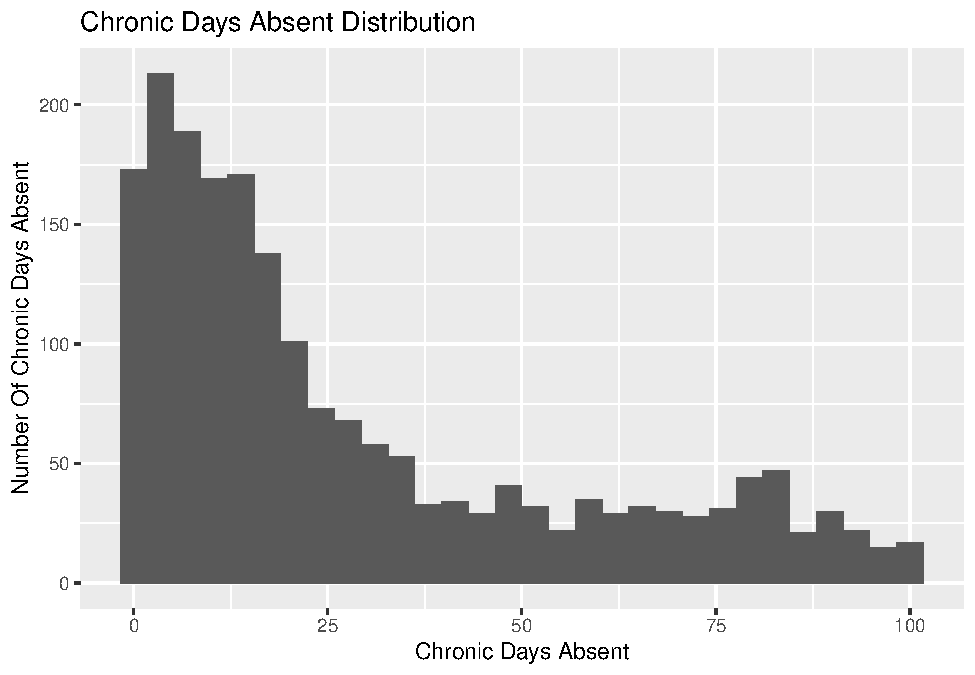
\includegraphics{final-writeup_files/figure-latex/unnamed-chunk-3-1.pdf}

\begin{verbatim}
## # A tibble: 1 x 5
##     max   min  mean   med    sd
##   <dbl> <dbl> <dbl> <dbl> <dbl>
## 1   100     0  28.4  17.4  27.6
\end{verbatim}

\begin{verbatim}
## `stat_bin()` using `bins = 30`. Pick better value with `binwidth`.
\end{verbatim}

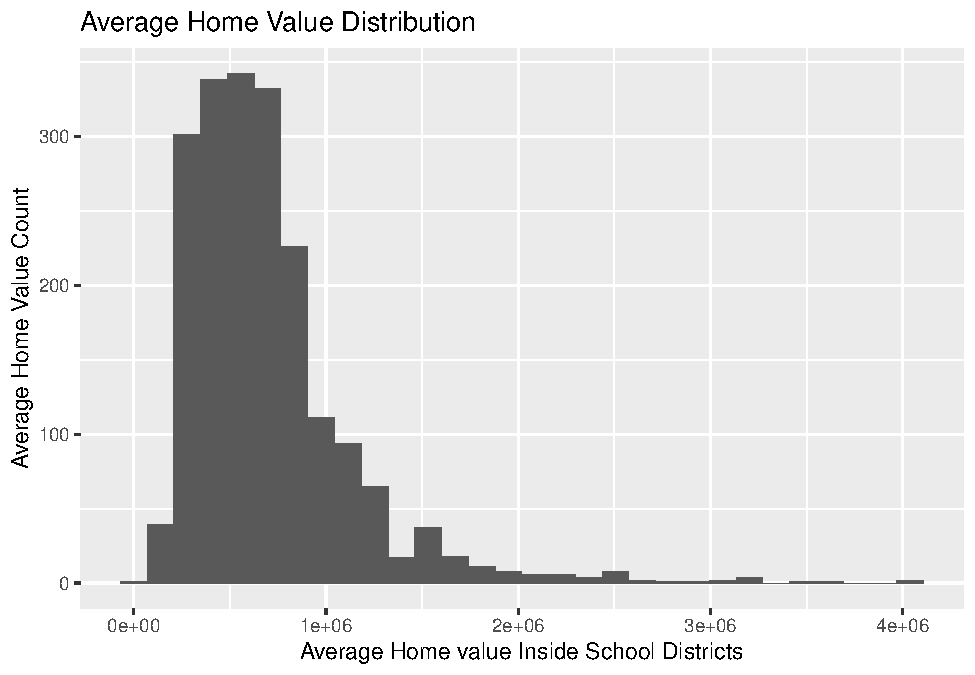
\includegraphics{final-writeup_files/figure-latex/unnamed-chunk-3-2.pdf}

\begin{verbatim}
## # A tibble: 1 x 5
##        max    min    mean     med      sd
##      <dbl>  <dbl>   <dbl>   <dbl>   <dbl>
## 1 4105966. 68073. 697944. 616592. 437134.
\end{verbatim}

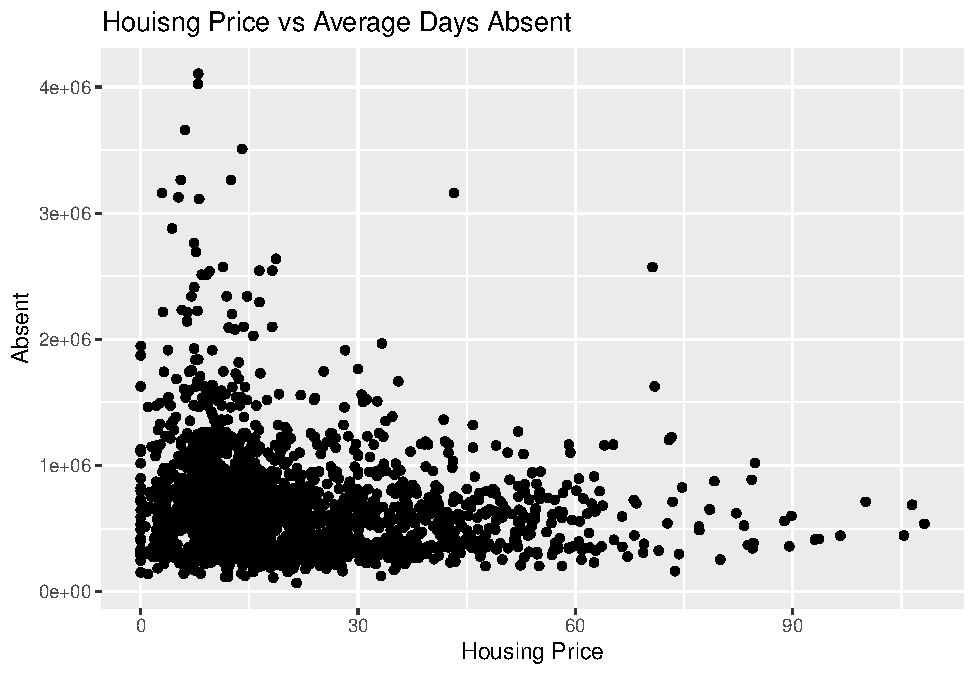
\includegraphics{final-writeup_files/figure-latex/unnamed-chunk-3-3.pdf}
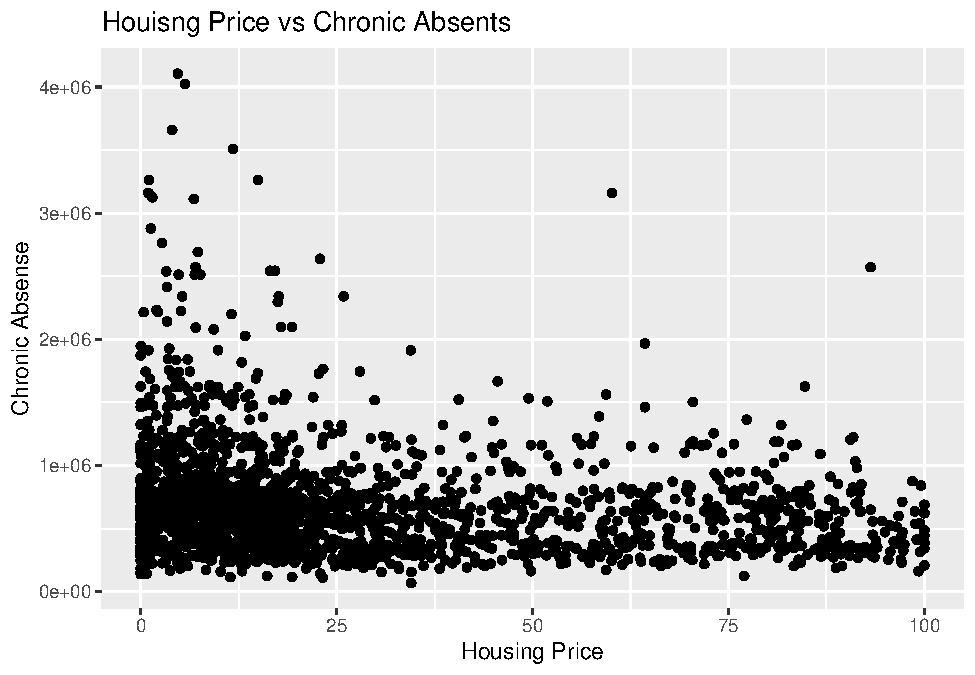
\includegraphics{final-writeup_files/figure-latex/unnamed-chunk-3-4.pdf}
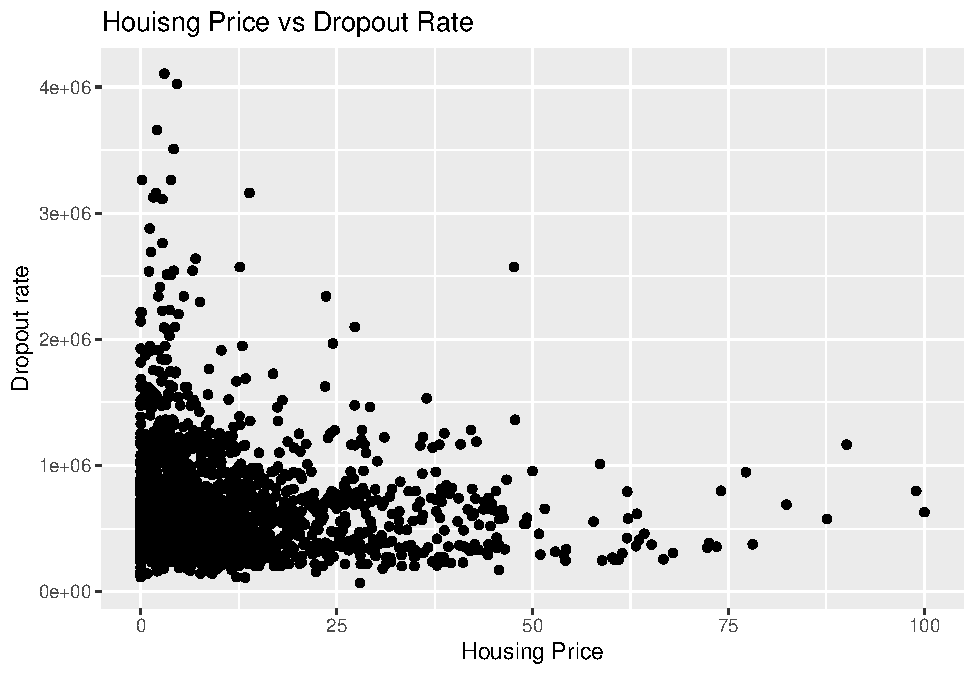
\includegraphics{final-writeup_files/figure-latex/unnamed-chunk-3-5.pdf}
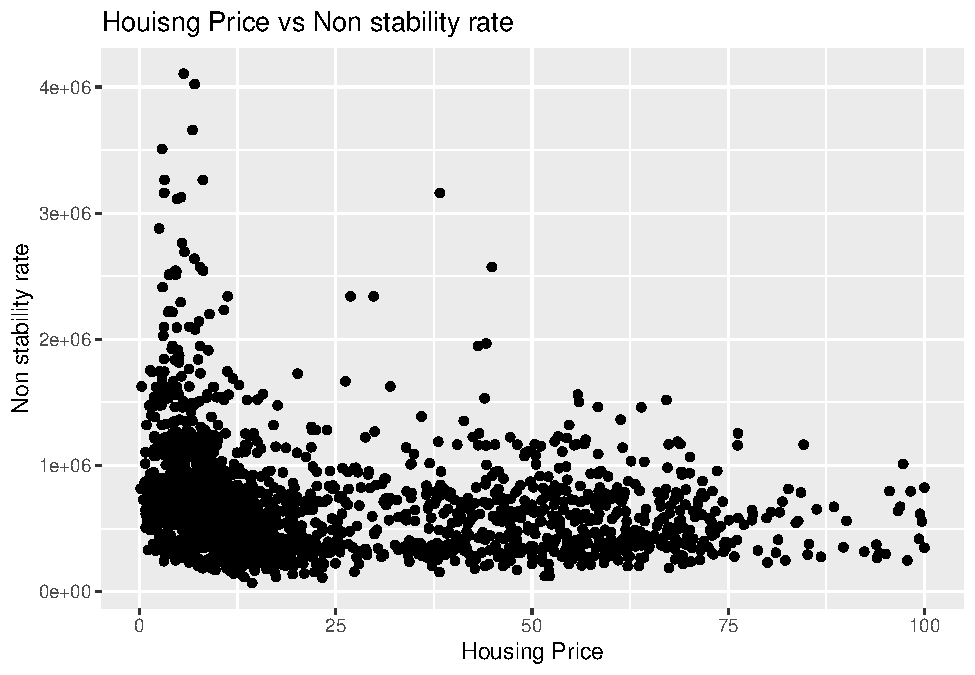
\includegraphics{final-writeup_files/figure-latex/unnamed-chunk-3-6.pdf}
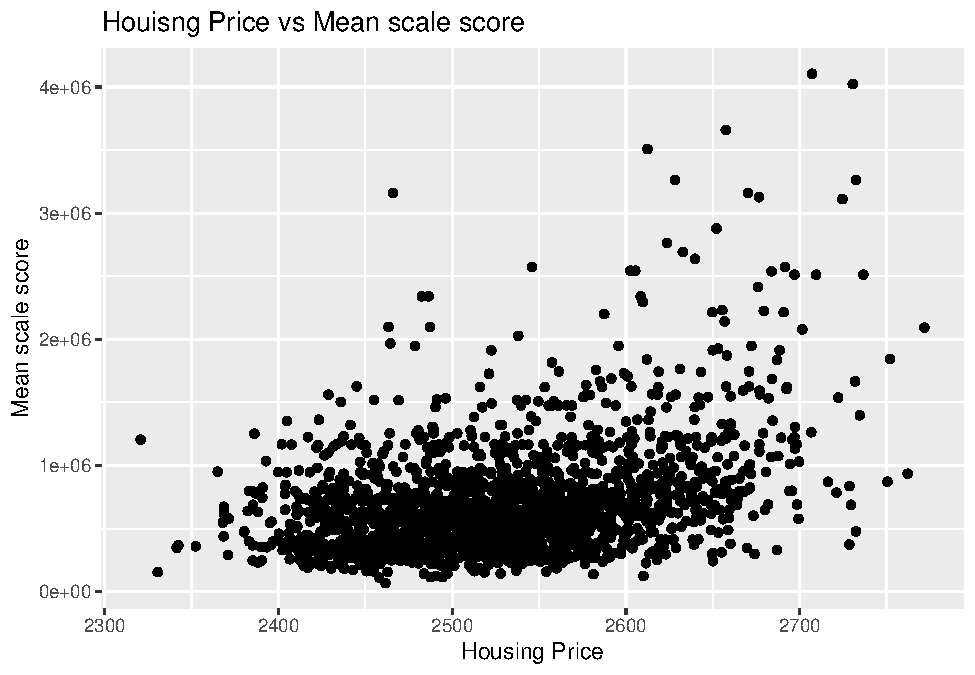
\includegraphics{final-writeup_files/figure-latex/unnamed-chunk-3-7.pdf}

During the folloowing section I scale the value of the houisng price by
taking the log of the value.

In the following place we create three models. The first model is all of
the values. The next one is without non stability rate. The next one is
suspension rate.

\begin{longtable}[]{@{}
  >{\raggedright\arraybackslash}p{(\columnwidth - 12\tabcolsep) * \real{0.3563}}
  >{\raggedleft\arraybackslash}p{(\columnwidth - 12\tabcolsep) * \real{0.1034}}
  >{\raggedleft\arraybackslash}p{(\columnwidth - 12\tabcolsep) * \real{0.1149}}
  >{\raggedleft\arraybackslash}p{(\columnwidth - 12\tabcolsep) * \real{0.1149}}
  >{\raggedleft\arraybackslash}p{(\columnwidth - 12\tabcolsep) * \real{0.0920}}
  >{\raggedleft\arraybackslash}p{(\columnwidth - 12\tabcolsep) * \real{0.1034}}
  >{\raggedleft\arraybackslash}p{(\columnwidth - 12\tabcolsep) * \real{0.1149}}@{}}
\toprule()
\begin{minipage}[b]{\linewidth}\raggedright
term
\end{minipage} & \begin{minipage}[b]{\linewidth}\raggedleft
estimate
\end{minipage} & \begin{minipage}[b]{\linewidth}\raggedleft
std.error
\end{minipage} & \begin{minipage}[b]{\linewidth}\raggedleft
statistic
\end{minipage} & \begin{minipage}[b]{\linewidth}\raggedleft
p.value
\end{minipage} & \begin{minipage}[b]{\linewidth}\raggedleft
conf.low
\end{minipage} & \begin{minipage}[b]{\linewidth}\raggedleft
conf.high
\end{minipage} \\
\midrule()
\endhead
(Intercept) & 5.777 & 0.005 & 1180.298 & 0.000 & 5.768 & 5.787 \\
\texttt{Average\ Days\ Absent} & 0.039 & 0.012 & 3.268 & 0.001 & 0.016 &
0.063 \\
ChronicAbsenteeismRate & -0.026 & 0.014 & -1.914 & 0.056 & -0.053 &
0.001 \\
\texttt{Dropout\ (Rate)} & 0.015 & 0.006 & 2.408 & 0.016 & 0.003 &
0.028 \\
\texttt{Non-Stability\ Rate\ (percent)} & -0.001 & 0.008 & -0.148 &
0.882 & -0.017 & 0.015 \\
\texttt{Suspension\ Rate\ (Total)} & -0.027 & 0.005 & -5.366 & 0.000 &
-0.037 & -0.017 \\
\texttt{Mean\ Scale\ Score} & 0.098 & 0.007 & 14.522 & 0.000 & 0.085 &
0.111 \\
\bottomrule()
\end{longtable}

\begin{longtable}[]{@{}
  >{\raggedright\arraybackslash}p{(\columnwidth - 12\tabcolsep) * \real{0.3171}}
  >{\raggedleft\arraybackslash}p{(\columnwidth - 12\tabcolsep) * \real{0.1098}}
  >{\raggedleft\arraybackslash}p{(\columnwidth - 12\tabcolsep) * \real{0.1220}}
  >{\raggedleft\arraybackslash}p{(\columnwidth - 12\tabcolsep) * \real{0.1220}}
  >{\raggedleft\arraybackslash}p{(\columnwidth - 12\tabcolsep) * \real{0.0976}}
  >{\raggedleft\arraybackslash}p{(\columnwidth - 12\tabcolsep) * \real{0.1098}}
  >{\raggedleft\arraybackslash}p{(\columnwidth - 12\tabcolsep) * \real{0.1220}}@{}}
\toprule()
\begin{minipage}[b]{\linewidth}\raggedright
term
\end{minipage} & \begin{minipage}[b]{\linewidth}\raggedleft
estimate
\end{minipage} & \begin{minipage}[b]{\linewidth}\raggedleft
std.error
\end{minipage} & \begin{minipage}[b]{\linewidth}\raggedleft
statistic
\end{minipage} & \begin{minipage}[b]{\linewidth}\raggedleft
p.value
\end{minipage} & \begin{minipage}[b]{\linewidth}\raggedleft
conf.low
\end{minipage} & \begin{minipage}[b]{\linewidth}\raggedleft
conf.high
\end{minipage} \\
\midrule()
\endhead
(Intercept) & 5.777 & 0.005 & 1180.591 & 0.000 & 5.768 & 5.787 \\
\texttt{Average\ Days\ Absent} & 0.040 & 0.012 & 3.425 & 0.001 & 0.017 &
0.062 \\
ChronicAbsenteeismRate & -0.027 & 0.012 & -2.214 & 0.027 & -0.051 &
-0.003 \\
\texttt{Dropout\ (Rate)} & 0.015 & 0.006 & 2.521 & 0.012 & 0.003 &
0.027 \\
\texttt{Suspension\ Rate\ (Total)} & -0.027 & 0.005 & -5.389 & 0.000 &
-0.037 & -0.017 \\
\texttt{Mean\ Scale\ Score} & 0.098 & 0.006 & 15.277 & 0.000 & 0.086 &
0.111 \\
\bottomrule()
\end{longtable}

\begin{longtable}[]{@{}
  >{\raggedright\arraybackslash}p{(\columnwidth - 12\tabcolsep) * \real{0.3563}}
  >{\raggedleft\arraybackslash}p{(\columnwidth - 12\tabcolsep) * \real{0.1034}}
  >{\raggedleft\arraybackslash}p{(\columnwidth - 12\tabcolsep) * \real{0.1149}}
  >{\raggedleft\arraybackslash}p{(\columnwidth - 12\tabcolsep) * \real{0.1149}}
  >{\raggedleft\arraybackslash}p{(\columnwidth - 12\tabcolsep) * \real{0.0920}}
  >{\raggedleft\arraybackslash}p{(\columnwidth - 12\tabcolsep) * \real{0.1034}}
  >{\raggedleft\arraybackslash}p{(\columnwidth - 12\tabcolsep) * \real{0.1149}}@{}}
\toprule()
\begin{minipage}[b]{\linewidth}\raggedright
term
\end{minipage} & \begin{minipage}[b]{\linewidth}\raggedleft
estimate
\end{minipage} & \begin{minipage}[b]{\linewidth}\raggedleft
std.error
\end{minipage} & \begin{minipage}[b]{\linewidth}\raggedleft
statistic
\end{minipage} & \begin{minipage}[b]{\linewidth}\raggedleft
p.value
\end{minipage} & \begin{minipage}[b]{\linewidth}\raggedleft
conf.low
\end{minipage} & \begin{minipage}[b]{\linewidth}\raggedleft
conf.high
\end{minipage} \\
\midrule()
\endhead
(Intercept) & 5.777 & 0.005 & 1172.066 & 0.000 & 5.768 & 5.787 \\
\texttt{Average\ Days\ Absent} & 0.049 & 0.012 & 4.102 & 0.000 & 0.025 &
0.072 \\
ChronicAbsenteeismRate & -0.036 & 0.014 & -2.642 & 0.008 & -0.062 &
-0.009 \\
\texttt{Dropout\ (Rate)} & 0.017 & 0.006 & 2.569 & 0.010 & 0.004 &
0.029 \\
\texttt{Non-Stability\ Rate\ (percent)} & -0.004 & 0.008 & -0.498 &
0.619 & -0.020 & 0.012 \\
\texttt{Mean\ Scale\ Score} & 0.098 & 0.007 & 14.461 & 0.000 & 0.085 &
0.112 \\
\bottomrule()
\end{longtable}

All the p values for the second regression model are below the .05. The
following is to check Normality and linearity. As you can see all but
regression model 1 accepts linearity condition and All follow Normality
condition. Independence is already accepted by how we collected the
data.

\begin{verbatim}
## `stat_bin()` using `bins = 30`. Pick better value with `binwidth`.
\end{verbatim}

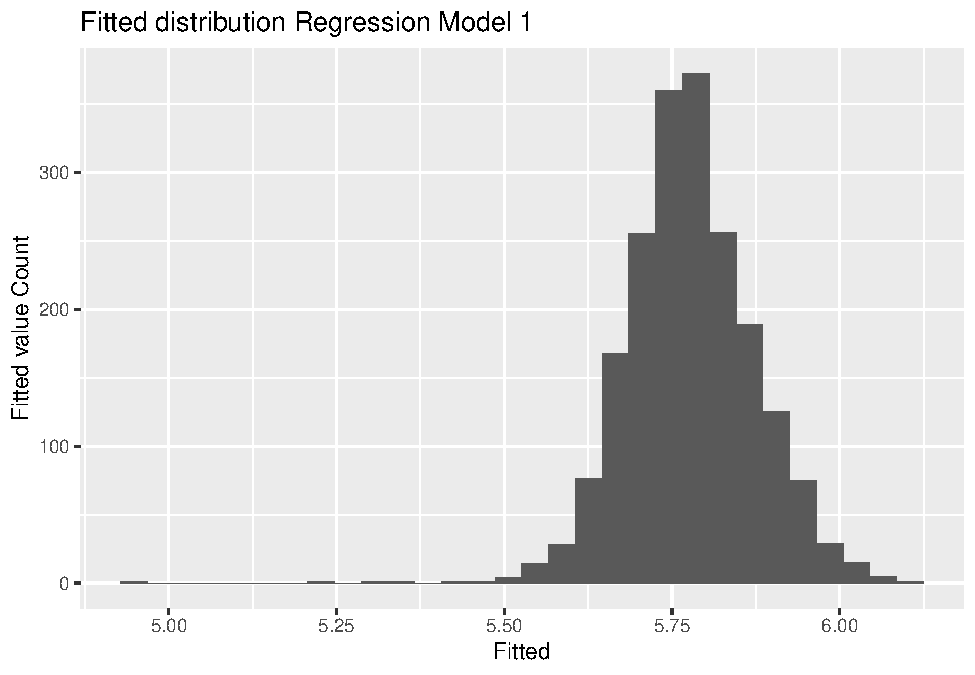
\includegraphics{final-writeup_files/figure-latex/unnamed-chunk-6-1.pdf}
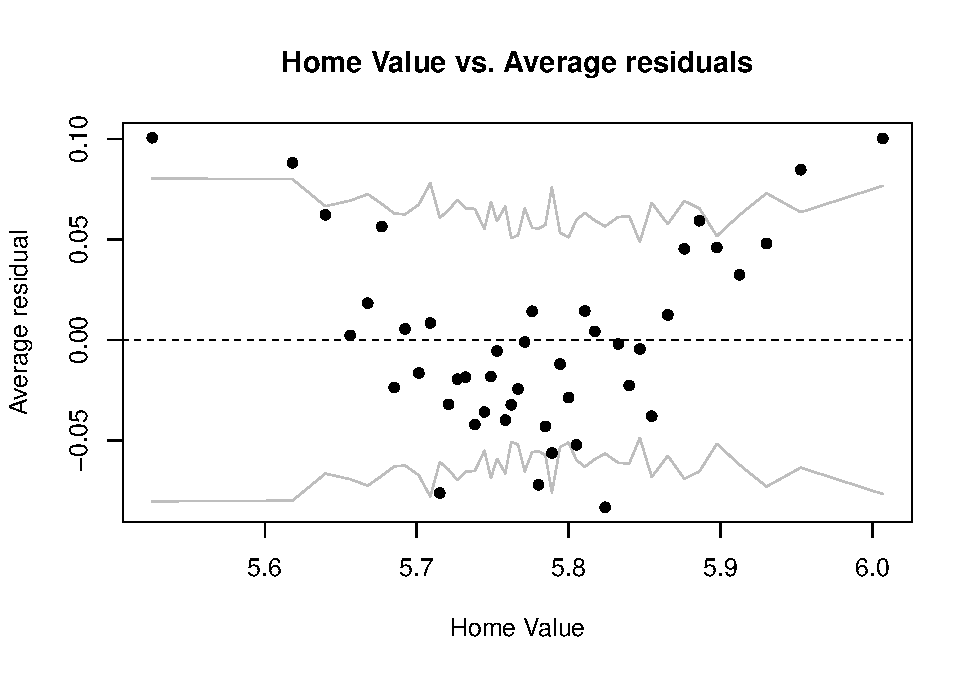
\includegraphics{final-writeup_files/figure-latex/unnamed-chunk-6-2.pdf}

\begin{verbatim}
## `stat_bin()` using `bins = 30`. Pick better value with `binwidth`.
\end{verbatim}

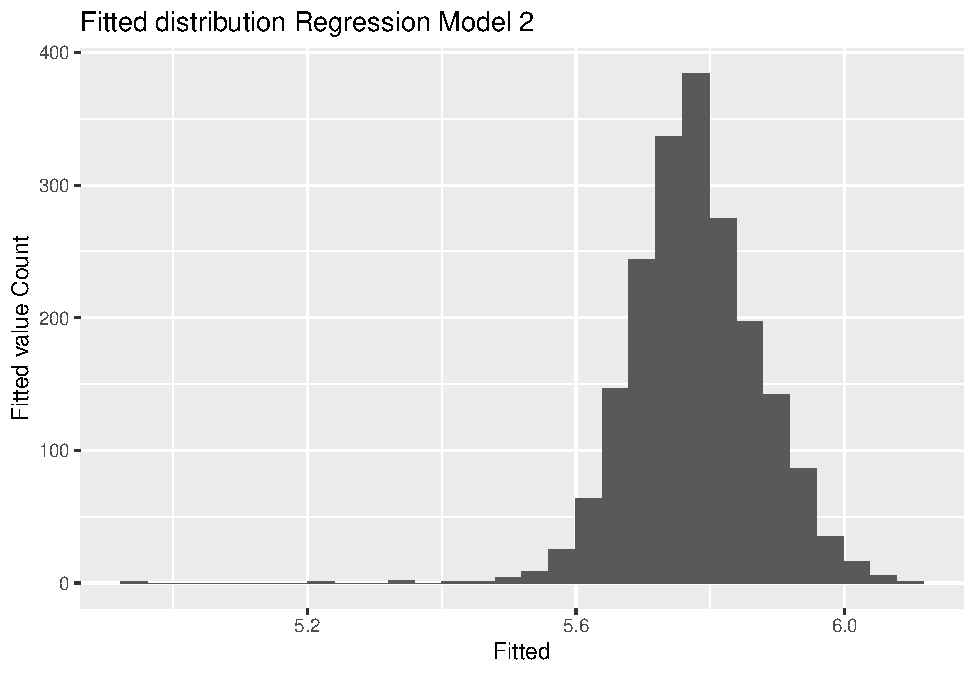
\includegraphics{final-writeup_files/figure-latex/unnamed-chunk-6-3.pdf}
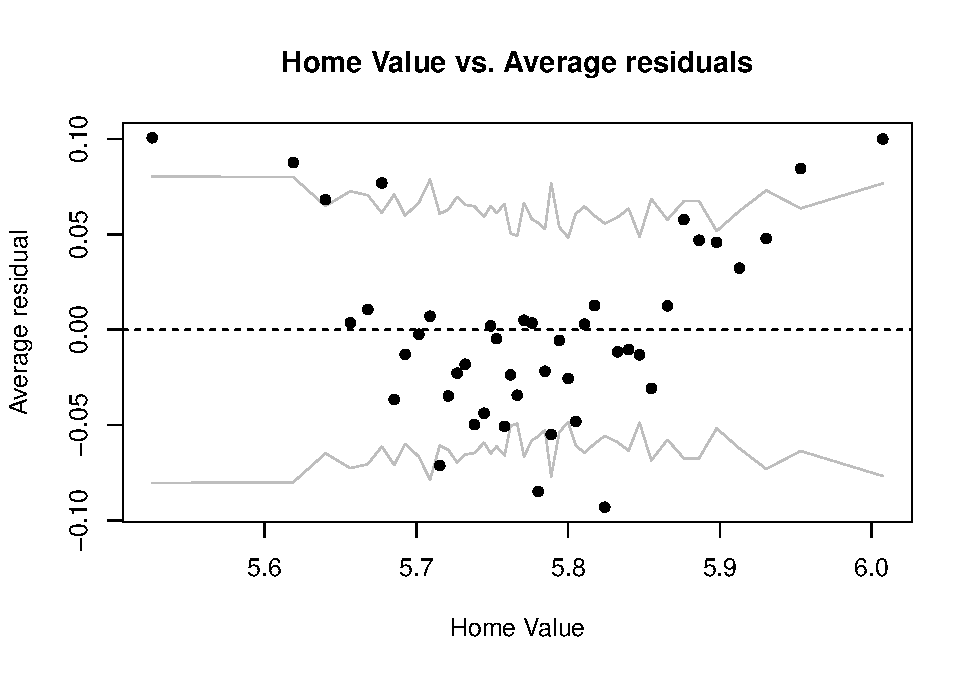
\includegraphics{final-writeup_files/figure-latex/unnamed-chunk-6-4.pdf}

\begin{verbatim}
## `stat_bin()` using `bins = 30`. Pick better value with `binwidth`.
\end{verbatim}

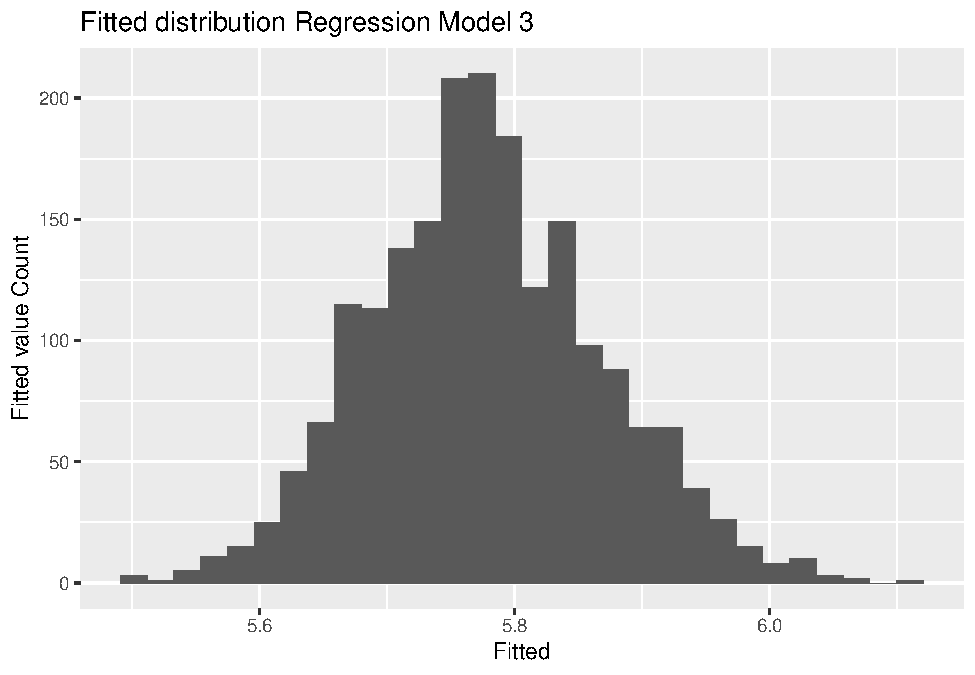
\includegraphics{final-writeup_files/figure-latex/unnamed-chunk-6-5.pdf}
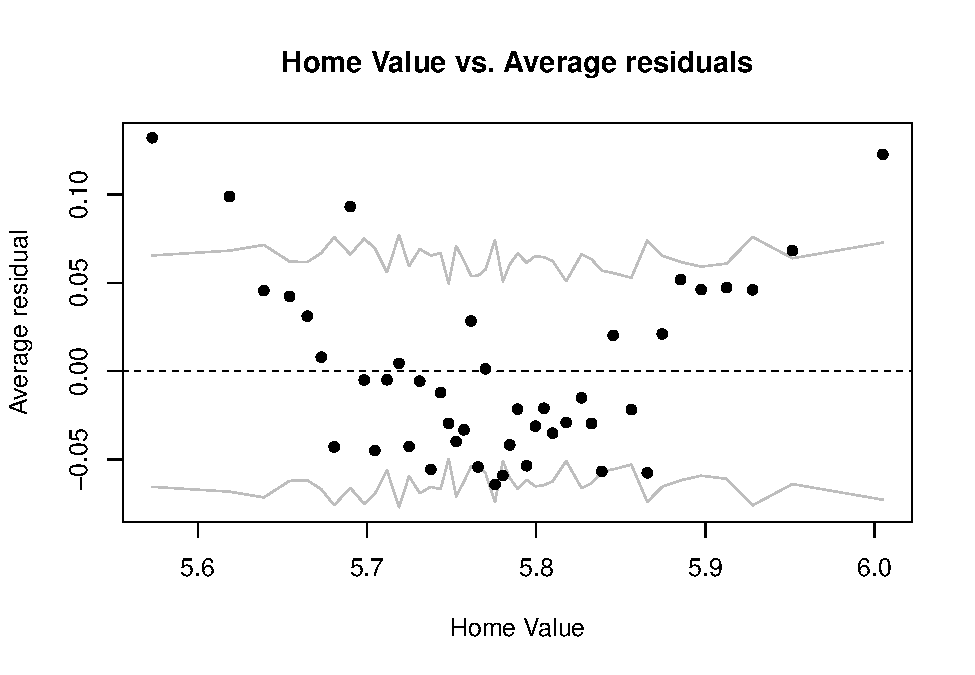
\includegraphics{final-writeup_files/figure-latex/unnamed-chunk-6-6.pdf}
Regression model 2 gives the following equation: 5.7710\^{}x0+.04(x1)+
-.027x2+.015\emph{x3-.027}x4+.098*x5. I preformed a couple of tests and
say the summary statsitics for the model such as the r square as well as
these showcase that values between 1 to 5 are somewhat corelated. Values
5+ are highly and 0 to 1 are not that correlated.

\begin{verbatim}
## Analysis of Variance Table
## 
## Model 1: average2021 ~ `Average Days Absent` + ChronicAbsenteeismRate + 
##     `Dropout (Rate)` + `Suspension Rate (Total)` + `Mean Scale Score`
## Model 2: average2021 ~ `Average Days Absent` + ChronicAbsenteeismRate + 
##     `Dropout (Rate)` + `Non-Stability Rate (percent)` + `Suspension Rate (Total)` + 
##     `Mean Scale Score`
##   Res.Df    RSS Df Sum of Sq Pr(>Chi)
## 1   1972 93.408                      
## 2   1971 93.407  1 0.0010422   0.8821
\end{verbatim}

\begin{verbatim}
## Analysis of Variance Table
## 
## Model 1: average2021 ~ `Average Days Absent` + ChronicAbsenteeismRate + 
##     `Dropout (Rate)` + `Non-Stability Rate (percent)` + `Mean Scale Score`
## Model 2: average2021 ~ `Average Days Absent` + ChronicAbsenteeismRate + 
##     `Dropout (Rate)` + `Non-Stability Rate (percent)` + `Suspension Rate (Total)` + 
##     `Mean Scale Score`
##   Res.Df    RSS Df Sum of Sq  Pr(>Chi)    
## 1   1972 94.772                           
## 2   1971 93.407  1    1.3647 8.037e-08 ***
## ---
## Signif. codes:  0 '***' 0.001 '**' 0.01 '*' 0.05 '.' 0.1 ' ' 1
\end{verbatim}

\begin{verbatim}
## 
## Call:
## lm(formula = average2021 ~ `Average Days Absent` + ChronicAbsenteeismRate + 
##     `Dropout (Rate)` + `Suspension Rate (Total)` + `Mean Scale Score`, 
##     data = data)
## 
## Residuals:
##      Min       1Q   Median       3Q      Max 
## -0.78714 -0.15120  0.00108  0.13974  0.95356 
## 
## Coefficients:
##                            Estimate Std. Error  t value Pr(>|t|)    
## (Intercept)                5.777310   0.004894 1180.591  < 2e-16 ***
## `Average Days Absent`      0.039549   0.011546    3.425 0.000626 ***
## ChronicAbsenteeismRate    -0.026874   0.012141   -2.214 0.026973 *  
## `Dropout (Rate)`           0.015139   0.006005    2.521 0.011774 *  
## `Suspension Rate (Total)` -0.026927   0.004997   -5.389 7.94e-08 ***
## `Mean Scale Score`         0.098471   0.006446   15.277  < 2e-16 ***
## ---
## Signif. codes:  0 '***' 0.001 '**' 0.01 '*' 0.05 '.' 0.1 ' ' 1
## 
## Residual standard error: 0.2176 on 1972 degrees of freedom
## Multiple R-squared:  0.1594, Adjusted R-squared:  0.1572 
## F-statistic: 74.76 on 5 and 1972 DF,  p-value: < 2.2e-16
\end{verbatim}

\begin{verbatim}
##     `Average Days Absent`    ChronicAbsenteeismRate          `Dropout (Rate)` 
##                  5.563722                  6.151946                  1.504836 
## `Suspension Rate (Total)`        `Mean Scale Score` 
##                  1.042037                  1.734102
\end{verbatim}

Doing a Chi square test on the Data where Null hypothesis is that the
variable removed is not a predictor and alternative hypothesis is that
it is a predictor we see that the chi square test we see that we accept
the null hypothesis and remove it from the test. Meaning the the second
model is best.

\begin{verbatim}
## [1] "average residual for the model is"
\end{verbatim}

\begin{verbatim}
## [1] -3.356257e-17
\end{verbatim}

There are a couple of limitations which should be noticed. One is that
there are only no enough observations to cover every school district
inside of california. The could make the model that we use not
applicable to the entirity of California. However a a large portion of
california is covered. Additionaly, many times it can be assumed that
schools arent represented are ones in lower income brackets. This could
cause a bit of bias onto the model itself. I additionally would also
like to add more variables which are applicable to the study I believe
that could greatly improve the accuracy of the model.
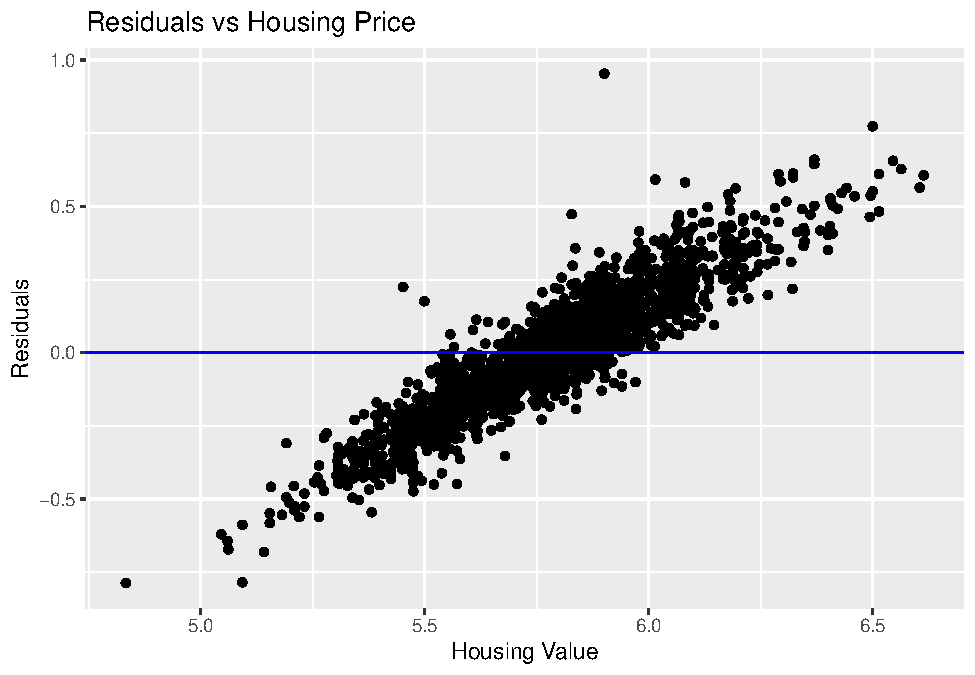
\includegraphics{final-writeup_files/figure-latex/unnamed-chunk-9-1.pdf}
Conclusion: There were a variety of models which I analyzed inside this
paper and more specifically I noticed some interesting results that were
to notice is that average days absence and dropout rate are both values
that increase the housing price when i expected them to decrease it.
This is a direct result of the different reasons these occur for rich
verus poor people. For example a poor person does not neccisarily have
the luxary of dropping out as they have little to no fall back plan
which is in their mind safe. While a rich person would have the support
of the parents so they are capable of making such a drastic result. Test
scores has the largest effect on home prices.

\end{document}
